\scanpage{62}

d'ordre \inserted{$d'$} divisant $d$, et a fortiori $d^t$.

c) \deleted{Pour tout} Soit $n$ un entier, et supposons que $n$ est premier à $p$, \uline{ou} que \inserted{$\unsure{d_t|d^t}$ est premier à $p$, ou que} $k$ est parfait(donc algébriquement clos).On a alors une suite exacte canonique, fonctorielle en $X$:
\diagram{\begin{tikzcd}[column sep=small]
(6)\quad 0\arrow[r]&{}_n\Gamma\arrow[r]\arrow[d,equal]&H^1(X,\mu_n)\arrow[r,"u_n"]&H^1(X_{\bar\eta},\mu_n)^I\arrow[r]&\operatorname{Ker}\deleted{{}_{\unsure{n}}}w_n\arrow[r]&0,\\
&\inserted{\underline Z/(n,d)\underline Z}&&&&
\end{tikzcd}}
où
\[
w_n:\Gamma_n\longrightarrow\operatorname{NS}(X_0)_n
\]
est l'homomorphisme déduit de (5) par tensorisation par $\underline Z/n\underline Z$, \deleted{Pour $n$ variable \unsure{multiplier}} et où $u_n$ est l'homomorphisme canonique (\qquad). Pour $n$ variable multiplicativement, les suites exactes (6) forment un système projectif de suites exactes, pour les morphismes de transition évidents.

\margin{$\times\quad\times\quad\times$}

d) Soit $\ell$ un nombre premier, \deleted{et supposons $\ell\neq p$ ou $k$ parfait.}\deleted{\inserted{ou $d_t$ premier à $p$ ou}} Alors on \deleted{trouve}\inserted{a} une suite exacte canonique, \inserted{fonctorielle en $X$} \deleted{(obtenue, si $\ell$ satisfait \inserted{aux conditions de c)}, par passage à la limite projective sur les puissances de $\ell$ dans les suites exactes (6)):}\deleted{on trouve une suite exacte}
\diagram{\begin{tikzcd}[column sep=small]
(7)\quad0\arrow[r,dash]&H^1(X,\underline Z_\ell(1))\arrow[r,"u(\ell)"]&H^1(X_{\bar\eta},\underline Z_\ell(1))^I\arrow[r]&R\otimes\underline Z_\ell\arrow[r]&0,
\end{tikzcd}}
où $R=\operatorname{Ker}w\simeq\underline Z/d'\underline Z$, donc
\[
(8)\qquad R\otimes\underline Z_\ell\simeq
\begin{cases}
0\text{ si }\ell\nmid d',\quad\inserted{\text{a fortiori si }\ell\nmid d^t,}\\
\underline Z/\ell\underline Z\text{ si }\ell\mid d'.
\end{cases}
\]
\margin{\figure{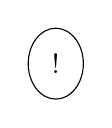
\begin{tikzpicture}\node at (0,0) {!};\draw (0,0) ellipse (.35 and .45);\end{tikzpicture}}}
\figure{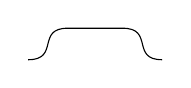
\begin{tikzpicture}\draw (0,0)..controls (.4,0) and (.1,.4)..(.5,.4)--(1.2,.4)..controls (1.6,.4) and (1.3,0)..(1.7,0);\end{tikzpicture}}

On obtient en particulier\unsure{*}, grâce à d): \deleted{du moins si $\ell\neq p$:}

\uline{Corollaire} \inserted{9}. \deleted{L'homomorphisme} Soit $\ell$ un nombre premier, \deleted{\unsure{tel que l'on ait $\ell\neq p$ si $k$ n'est pas parfait ou $d_t$}} Alors l'homomorphisme
\[
\inserted{(10)}\qquad u(\ell):H^1(X,\underline Z_\ell(1))\longrightarrow H^1(X_{\bar\eta},\underline Z_\ell(1))^I
\]
est injectif, son conoyau est un groupe fini, nul pour presque tout $\ell$.
La même conclusion est vraie en remplaçant $\underline Z_\ell(1)$ par $\underline Z_\ell$, à condition de supposer $\ell\neq p$.

\margin{$\times$}
\margin{\figure{\begin{tikzpicture}\draw (0,8)--(0,0);\draw (.2,-1)--(.2,-3);\end{tikzpicture}}}
\margin{61}
